% --- chapter
\newcommand{\chapter}[2][]{
	\newcommand{\chapname}{#2}
	\begin{flushleft}
		\begin{minipage}[t]{\linewidth}
			
\includegraphics[height=1cm]{hdht-logo.png}
			\hspace{0pt}	
			\sffamily\bfseries\large Bài  28. Tia X
			\begin{flushleft}
				\huge\bfseries #1
			\end{flushleft}
		\end{minipage}
	\end{flushleft}
	\vspace{1cm}
	\normalfont\normalsize
}
%-----------------------------------------------------
\chapter[Tia X]{Tia X}

\subsection{Bản chất}

Tia X (còn gọi là tia R\"ontgen) là sóng điện từ có bước sóng rất ngắn (từ $10^{-8}\ \text{m}$ đến $10^{-11}\ \text{m}$).

\subsection {Cách tạo ra}
Tia X được tạo thành từ ống phóng tia X:
\begin{itemize}
\item Các electron từ cathode được tăng tốc trong điện trường mạnh sẽ có động năng lớn.
\item Khi electron đập vào đối cathode, chúng xuyên qua lớp vỏ nguyên tử, tương tác với hạt nhân và các electron ở bên trong làm phát ra sóng điện từ có bước sóng cực ngắn, gọi là tia X.

\begin{center}
	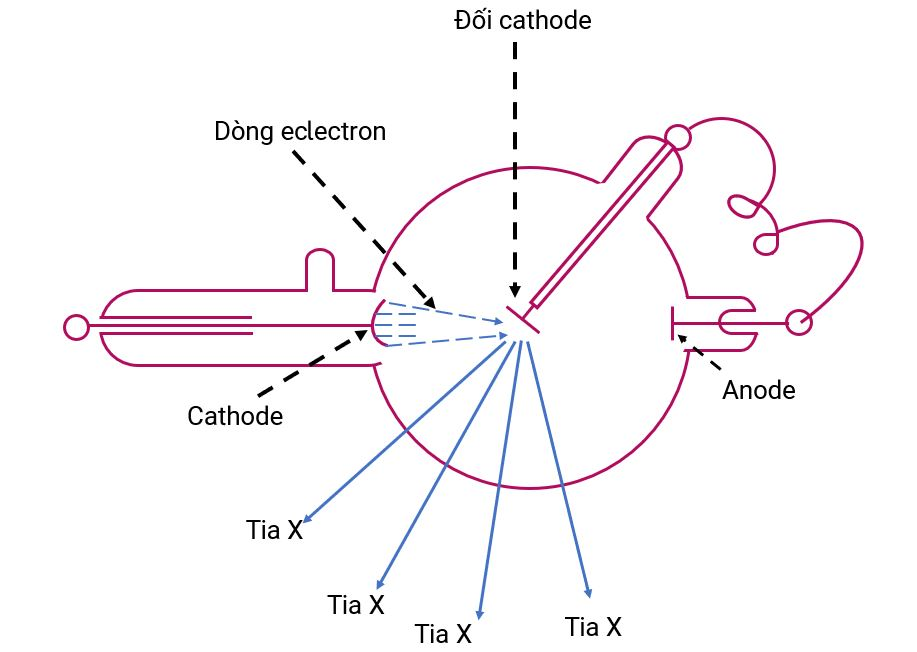
\includegraphics[scale=0.5]{../figs/VN12-PH-36-L-021-5-1.JPG}
\end{center}
\end{itemize}
Ngoài ra, tia X còn được tạo thành do quá trình va chạm trong các khối khí có nhiệt độ rất cao (Mặt trời, các sao,...)
\subsection{Tính chất}

Tia X có các tính chất:

\begin{itemize}
	\item Tính chất nổi bật nhất là khả năng đâm xuyên qua giấy, vải, gỗ thậm chí cả kim loại. Tia X có bước sóng càng ngắn thì càng xuyên được sâu hay càng cứng.
	\item Tác dụng mạnh lên kính ảnh.
	\item Làm ion hóa không khí. 
	\item Làm phát quang một số chất.
	\item Tác dụng sinh lý: làm hủy họa tế bào, diệt vi khuẩn,..
	
\end{itemize}

\subsection{Ứng dụng}

\begin{itemize}
	\item Y học: sử dụng để chiếu điện, chụp điện, chữa ung thư nông.
	\item Công nghiệp: kiểm tra chất lượng bên trong sản phẩm.
	\item Giao thông: kiểm tra hành lý của hành khách.
	\item Phòng thí nghiệm: nghiên cứu cấu trúc vật rắn.
\end{itemize}
